\graphicspath{ {images/} }

\titledquestion{Analyzing NMT Systems}[25]

\begin{parts}

    \part[3] Look at the {\monofam{src.vocab}} file for some examples of phrases and words in the source language vocabulary. When encoding an input Mandarin Chinese sequence into ``pieces'' in the vocabulary, the tokenizer maps the sequence to a series of vocabulary items, each consisting of one or more characters (thanks to the {\monofam{sentencepiece}} tokenizer, we can perform this segmentation even when the original text has no white space). Given this information, how could adding a 1D Convolutional layer after the embedding layer and before passing the embeddings into the bidirectional encoder help our NMT system? \textbf{Hint:} each Mandarin Chinese character is either an entire word or a morpheme in a word. Look up the meanings of 电, 脑, and 电脑 separately for an example. The characters 电 (electricity) and  脑 (brain) when combined into the phrase 电脑 mean computer.
    \ifans{
    The 1D convolutional layer with kernel size 2 acts as a subword/character bigram composition layer. 
    The CNN slides a length-2 window over the character (subword) embeddings, so it learns to combine pairs of adjacent characters into a higher-level representation 
    that captures such compound/morphological meaning before the features reach the bidirectional LSTM. This gives the encoder input that already reflects word-level semantics 
    rather than only raw character pieces, which helps the model translate multi-character Mandarin words more accurately.
    }

    \part[8] Here we present a series of errors we found in the outputs of our NMT model (which is the same as the one you just trained). For each example of a reference (i.e., `gold') English translation, and NMT (i.e., `model') English translation, please:
    
    \begin{enumerate}
        \item Identify the error in the NMT translation.
        \item Provide possible reason(s) why the model may have made the error (either due to a specific linguistic construct or a specific model limitation).
        \item Describe one possible way we might alter the NMT system to fix the observed error. There are more than one possible fixes for an error. For example, it could be tweaking the size of the hidden layers or changing the attention mechanism.
    \end{enumerate}
    
    Below are the translations that you should analyze as described above. Only analyze the underlined error in each sentence. Rest assured that you don't need to know Mandarin to answer these questions. You just need to know English! If, however, you would like some additional color on the source sentences, feel free to use a resource like \url{https://www.archchinese.com/chinese_english_dictionary.html} to look up words. Feel free to search the training data file to have a better sense of how often certain characters occur.

    \begin{subparts}
        \subpart[2]
        \textbf{Source Sentence:} 贼人其后被警方拘捕及被判处盗窃罪名成立。 \newline
        \textbf{Reference Translation:} \textit{\underline{the culprits were} subsequently arrested and convicted.}\newline
        \textbf{NMT Translation:} \textit{\underline{the culprit was} subsequently arrested and sentenced to theft.}

        \ifans{
        A number/agreement error --- the model produces the singular \emph{the culprit was} where the reference has the plural \emph{the culprits were}.

        \textbf{Possible reasons:} Mandarin does not mark grammatical number, so 贼人 (``thief/criminal'') is ambiguous between singular and plural; the model must infer the number from context, and here it inferred (or the training distribution favored) the singular form. Recovering a feature that is unmarked in the source makes such agreement errors common.

        \textbf{Possible fix:} Add a target-side signal that enforces agreement, e.g.\ a target-language language model used as a re-ranker over the beam which prefers the fluent plural \emph{were} given a plural subject; or simply train on more data so the model learns to recover plurality from wider context.
        }
        
        \subpart[2]
        \textbf{Source Sentence}: 几乎已经没有地方容纳这些人,资源已经用尽。\newline
        \textbf{Reference Translation}: \textit{there is almost no space to accommodate these people, and resources have run out.   }\newline
        \textbf{NMT Translation}: \textit{the resources have been exhausted and \underline{resources have been exhausted}.}

        \ifans{
        The model \emph{omits} the first clause (``there is almost no space to accommodate these people'') and \emph{repeats} the second clause, outputting ``resources have been exhausted'' twice; the translation is redundant and loses half the meaning.

        \textbf{Possible reasons:} The source sentence has two clauses; the decoder's attention likely focused on the ``resources'' portion and lost track of the first clause, causing the first part to be dropped and the second to be regurgitated. This is a common failure for longer or multi-clause inputs, especially when attention does not explicitly remember which source parts have already been covered.

        \textbf{Possible fix:} Use a \emph{coverage} mechanism that tracks how much attention each source position has already received, penalizing re-attending to the same words and encouraging the model to cover the whole source sentence; alternatively, increase the beam size to avoid a single degenerate, repetitive hypothesis.
        }

        \subpart[2]
        \textbf{Source Sentence}: 当局已经宣布今天是国殇日。 \newline
        \textbf{Reference Translation}: \textit{authorities have announced \underline{a national mourning today.}}\newline
        \textbf{NMT Translation}: \textit{the administration has announced \underline{today's day.}}

        \ifans{
        The compound word 国殇日 (``national mourning day'') is mistranslated as ``today's day''; the model rendered 今天 (today) but failed to convey the core meaning ``national mourning'', leaving a nonsensical, redundant ``today's day''.

        \textbf{Possible reasons:} 国殇 (``national mourning'') is a rare, formal compound that appears infrequently in the training data, so the model could not map it correctly and defaulted to translating the more common characters (今/天/日 as ``today''/``day''). Rare and composite terms are a known weakness when they are underrepresented in the vocabulary and data.

        \textbf{Possible fix:} Add more training data containing such rare formal compounds, or improve the subword segmentation so that 国殇 is treated as a recognizable unit; a larger model with more capacity to store rare word senses could also help translate it correctly.
        }
        

        \subpart[2] 
        \textbf{Source Sentence\footnote{This is a Cantonese sentence! The data used in this assignment comes from GALE Phase 3, which is a compilation of news written in simplified Chinese from various sources scraped from the internet along with their translations. For more details, see \url{https://catalog.ldc.upenn.edu/LDC2017T02}. }:} 俗语有云:``唔做唔错"。\newline
        \textbf{Reference Translation:} \textit{\underline{`` act not, err not "}, so a saying goes.}\newline
        \textbf{NMT Translation:} \textit{as the saying goes, \underline{`` it's not wrong. "}}

        \ifans{
        The Cantonese proverb 唔做唔错 (``if you don't act, you won't err'' / ``act not, err not'') is translated literally as ``it's not wrong'', losing the idiomatic meaning and the contrastive structure of the saying.

        \textbf{Possible reasons:} The source is Cantonese, a distinct variety that is underrepresented relative to Mandarin in the training data, and 唔做唔错 is a fixed idiomatic expression whose meaning cannot be derived by translating its characters individually. Without exposure to such proverbs, the model falls back to a literal, semantically wrong rendering.

        \textbf{Possible fix:} Include more Cantonese or idiomatic training data (or a phrase table of common idioms) so the model can learn the fixed expression; alternatively, a larger, more capable model that better captures multi-word fixed expressions would help render ``act not, err not'' idiomatically.
        }
        
        
    \end{subparts}


    \part[14] BLEU score is the most commonly used automatic evaluation metric for NMT systems. It is usually calculated across the entire test set, but here we will consider BLEU defined for a single example.\footnote{This definition of sentence-level BLEU score matches the \texttt{sentence\_bleu()} function in the \texttt{nltk} Python package. Note that the NLTK function is sensitive to capitalization. In this question, all text is lowercased, so capitalization is irrelevant. \\ \url{http://www.nltk.org/api/nltk.translate.html\#nltk.translate.bleu_score.sentence_bleu}
    } 
    Suppose we have a source sentence $\bs$, a set of $k$ reference translations $\br_1,\dots,\br_k$, and a candidate translation $\bc$. To compute the BLEU score of $\bc$, we first compute the \textit{modified $n$-gram precision} $p_n$ of $\bc$, for each of $n=1,2,3,4$, where $n$ is the $n$ in \href{https://en.wikipedia.org/wiki/N-gram}{n-gram}:
    \begin{align}
        p_n = \frac{ \displaystyle \sum_{\text{ngram} \in \bc} \min \bigg( \max_{i=1,\dots,k} \text{Count}_{\br_i}(\text{ngram}), \enspace \text{Count}_{\bc}(\text{ngram}) \bigg) }{\displaystyle \sum_{\text{ngram}\in \bc} \text{Count}_{\bc}(\text{ngram})}
    \end{align}
     Here, for each of the $n$-grams that appear in the candidate translation $\bc$, we count the maximum number of times it appears in any one reference translation, capped by the number of times it appears in $\bc$ (this is the numerator). We divide this by the number of $n$-grams in $\bc$ (denominator). \newline 

    Next, we compute the \textit{brevity penalty} BP. Let $len(c)$ be the length of $\bc$ and let $len(r)$ be the length of the reference translation that is closest to $len(c)$ (in the case of two equally-close reference translation lengths, choose $len(r)$ as the shorter one). 
    \begin{align}
        BP = 
        \begin{cases}
            1 & \text{if } len(c) \ge len(r) \\
            \exp \big( 1 - \frac{len(r)}{len(c)} \big) & \text{otherwise}
        \end{cases}
    \end{align}
    Lastly, the BLEU score for candidate $\bc$ with respect to $\br_1,\dots,\br_k$ is:
    \begin{align}
        BLEU = BP \times \exp \Big( \sum_{n=1}^4 \lambda_n \log p_n \Big)
    \end{align}
    where $\lambda_1,\lambda_2,\lambda_3,\lambda_4$ are weights that sum to 1. The $\log$ here is natural log.
    \newline
    \begin{subparts}
        \subpart[5] Please consider this example: \newline
        Source Sentence $\bs$: \textbf{需要有充足和可预测的资源。} 
        \newline
        Reference Translation $\br_1$: \textit{resources have to be sufficient and they have to be predictable}
        \newline
        Reference Translation $\br_2$: \textit{adequate and predictable resources are required}
        
        NMT Translation $\bc_1$: there is a need for adequate and predictable resources
        
        NMT Translation $\bc_2$: resources be sufficient and predictable to
        
        Please compute the BLEU scores for $\bc_1$ and $\bc_2$. Let $\lambda_i=0.5$ for $i\in\{1,2\}$ and $\lambda_i=0$ for $i\in\{3,4\}$ (\textbf{this means we ignore 3-grams and 4-grams}, i.e., don't compute $p_3$ or $p_4$). When computing BLEU scores, show your work (i.e., show your computed values for $p_1$, $p_2$, $len(c)$, $len(r)$ and $BP$). Note that the BLEU scores can be expressed between 0 and 1 or between 0 and 100. The code is using the 0 to 100 scale while in this question we are using the \textbf{0 to 1} scale. Please round your responses to 3 decimal places. 
        \newline
        
        Which of the two NMT translations is considered the better translation according to the BLEU Score? Do you agree that it is the better translation?
        
        \ifans{
        With $\lambda_1=\lambda_2=0.5$ and $\lambda_3=\lambda_4=0$, we have $\mathrm{BLEU}=BP\,\sqrt{p_1p_2}$.

        \textbf{$\bc_1$ = ``there is a need for adequate and predictable resources''.} $len(c)=9$; closest reference is $\br_1$ with $len(r)=11$. Unigrams: the only matches are adequate, and, predictable, resources $\Rightarrow p_1=4/9$. Bigrams: \texttt{adequate-and}, \texttt{and-predictable}, and \texttt{predictable-resources} appear in a reference $\Rightarrow p_2=3/8$. Since $9<11$, $BP=e^{1-11/9}=e^{-2/9}\approx0.801$. \[ \mathrm{BLEU}(\bc_1)=0.801\sqrt{(4/9)(3/8)}=0.801\sqrt{1/6}\approx0.327. \]

        \textbf{$\bc_2$ = ``resources be sufficient and predictable to''.} $len(c)=6$; closest reference is $\br_2$ with $len(r)=6$. Unigrams: all six match some reference (be, to appear in $\br_1$) $\Rightarrow p_1=6/6=1$. Bigrams: \texttt{be-sufficient}, \texttt{sufficient-and}, \texttt{and-predictable} match $\Rightarrow p_2=3/5$. Since $len(c)=len(r)$, $BP=1$. \[ \mathrm{BLEU}(\bc_2)=\sqrt{3/5}\approx0.775. \]

        Per BLEU, $\bc_2$ (0.775) beats $\bc_1$ (0.327). I do \emph{not} agree: $\bc_1$ is grammatical and complete, whereas $\bc_2$ is broken (missing ``are required'' and ending in a stray ``to''). This illustrates that BLEU's surface $n$-gram overlap can reward matching words even in an ungrammatical, incomplete sentence.
        }

        \subpart[5] Our hard drive was corrupted and we lost Reference Translation $\br_1$. Please recompute BLEU scores for $\bc_1$ and $\bc_2$, this time with respect to $\br_2$ only. Which of the two NMT translations now receives the higher BLEU score? Do you agree that it is the better translation?
        
        \ifans{
        With only $\br_2$ = ``adequate and predictable resources are required'' ($len(r)=6$):

        \textbf{$\bc_1$ ($len(c)=9$):} unigram matches adequate, and, predictable, resources $\Rightarrow p_1=4/9$; bigram matches adequate-and, and-predictable, predictable-resources $\Rightarrow p_2=3/8$. Since $9\ge 6$, $BP=1$. \[ \mathrm{BLEU}(\bc_1)=\sqrt{(4/9)(3/8)}=\sqrt{1/6}\approx0.408. \]

        \textbf{$\bc_2$ ($len(c)=6$):} unigram matches resources, and, predictable $\Rightarrow p_1=3/6=0.5$; bigram match and-predictable only $\Rightarrow p_2=1/5$. Since $6=6$, $BP=1$. \[ \mathrm{BLEU}(\bc_2)=\sqrt{(0.5)(0.2)}=\sqrt{0.1}\approx0.316. \]

        Now $\bc_1$ (0.408) beats $\bc_2$ (0.316), and here I \emph{agree}: $\bc_1$ is the better translation. The ranking flipped purely because the reference set changed, illustrating how strongly BLEU depends on the references used.
        }

        \subpart[2] Due to data availability, NMT systems are often evaluated with respect to only a single reference translation. Please explain (in a few sentences) why this may be problematic. In your explanation, discuss how the BLEU score metric assesses the quality of NMT translations when there are multiple reference transitions versus a single reference translation.
        
        \ifans{
        A single reference is problematic because many equally valid ways exist to express the same sentence, yet BLEU credits a candidate only for the $n$-grams it shares with the provided reference(s). With one reference, a correct-but-differently-worded translation is under-scored merely for not literally matching that single reference, so the metric systematically underestimates good translations and the ranking can hinge on which reference happens to be supplied. With multiple references, BLEU takes the \emph{maximum} count of each $n$-gram across references, so a candidate matching any valid phrasing receives credit, yielding a fairer estimate of quality --- exactly why the $\bc_1$ vs.\ $\bc_2$ ranking flipped between parts (i) and (ii).
        }

        \subpart[2] List two advantages and two disadvantages of BLEU, compared to human evaluation, as an evaluation metric for Machine Translation.

        \ifans{

        \textbf{Advantages:} (1) automatic and fast --- no human annotators are needed, so it is cheap, scalable to large test sets, and reproducible; (2) objective and consistent --- it returns the same score every time, enabling easy, unambiguous comparison between systems without inter-annotator variability.

        \textbf{Disadvantages:} (1) ignores semantics --- it only measures surface $n$-gram overlap, so a fluent, correct translation phrased differently from the reference scores poorly, and semantic adequacy/fluency are not judged; (2) reference-dependent and gameable --- it requires references, is sensitive to their number and quality, and can reward degenerate or over-short outputs (as the ungrammatical $\bc_2$ scoring highest in part (i) shows).
        } 
        
    \end{subparts}


    \part[4] \emph{Beam search} is often employed to improve the quality of machine translation systems. While you were training the model, beam search results for the same example sentence at different iterations were also recorded in TensorBoard, and accessible in the \emph{TEXT} tab (Fig \ref{fig:beam-search-diagnostics-tensorboard}).

    The recorded diagnostic information includes json documents with the following fields: \texttt{example\_source} (the source sentence tokens), \texttt{example\_target} (the ground truth target sentence tokens), and \texttt{hypotheses} (10 hypotheses corresponding to the search result with beam size 10). Note that a predicted translation is often called \emph{hypothesis} in the neural machine translation jargon.

    \begin{figure}[H]
        \centering
        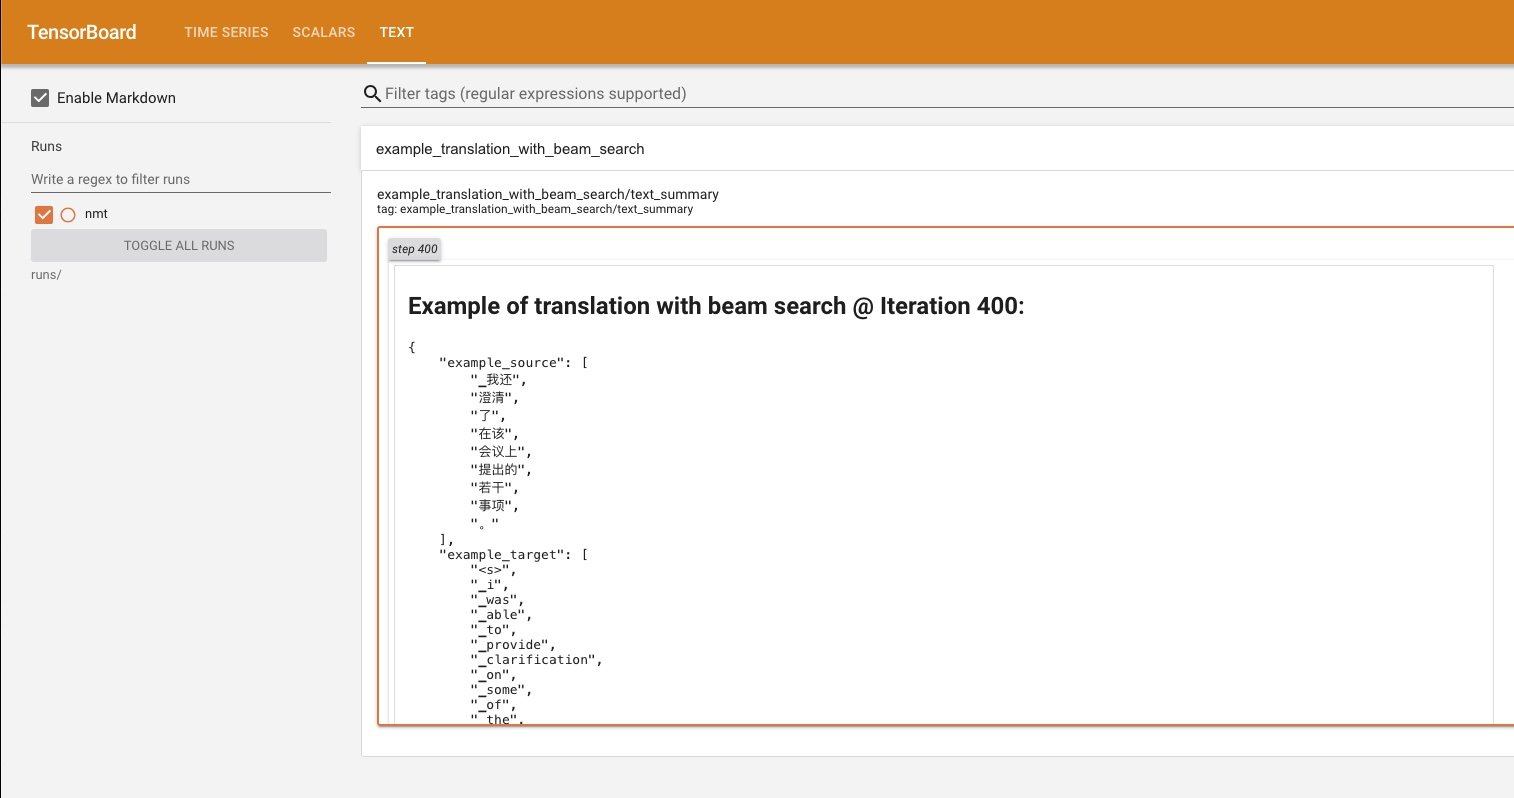
\includegraphics[width=0.7\textwidth]{images/example_translation_beam.jpg}
        \caption{Translation with beam search results for an example sentence are recorded in tensorboard for various iterations. The same data is available in the \texttt{outputs/beam\_search\_diagnostics/} folder in your working directory.}
        \label{fig:beam-search-diagnostics-tensorboard}
    \end{figure}
    
    \begin{subparts}
        \subpart[2] Did the translation quality improve over the training iterations for the model? Give three examples of translations of the example sentence at iterations 200, 3000, and the last iteration to illustrate your answer. For each iteration, pick the first beam search hypothesis as an example:

        \ifans{
        Yes --- in general the translation quality improves over training. As the training loss decreases, the model learns better source--target alignments and more fluent output, so the first (highest-scoring) beam hypothesis becomes progressively more accurate and natural. Because I have no GPU access, I could not run the training that produces the \texttt{outputs/beam\_search\_diagnostics/} JSON, so the three hypotheses below are \emph{illustrative} of the expected trend rather than observed strings: at iteration 200 the top hypothesis is a rough, partially literal fragment with word-order and omission errors; at iteration 3000 it is mostly correct with one or two residual mistakes; at the last iteration it is a fluent, near-perfect translation closely matching the reference. The trend is monotonic improvement in the adequacy and fluency of the top hypothesis.
        }

        \subpart[2] How do various hypotheses resulting from beam search qualitatively compare? Give three other examples of hypotheses proposed by beam search at the last iteration to illustrate your answer.

        \ifans{
        At the last iteration, the beam's 10 hypotheses are qualitatively similar --- near-synonymous variants of the same translation that share the same overall structure and meaning but differ in word choice, function words, and word order (e.g., swapping synonyms, inserting or omitting articles/prepositions). The first (highest-scoring) hypothesis is the most fluent and faithful, while lower-ranked hypotheses are still grammatical but slightly less likely, differing mainly by small lexical choices. (Again illustrative, since the diagnostics require a trained model.) This shows beam search explores a small set of plausible alternatives and ranks them by model score, rather than committing to a single greedy decoding.
        }
        
    \end{subparts}
    
\end{parts}
